\documentclass[12pt,a4paper]{report}

% ---------- Paket dasar ----------
\usepackage[utf8]{inputenc}
\usepackage[T1]{fontenc}
\usepackage[indonesian]{babel}
\usepackage{lipsum}

% ---------- Paket matematika & gambar ----------
\usepackage{amsmath,amssymb}
\usepackage{graphicx}
\usepackage{caption}
\usepackage{subcaption}
\usepackage{float}
\usepackage{tikz}
\usetikzlibrary{automata,positioning,arrows,shapes.geometric}
\bibliographystyle{IEEEtran}
% ---------- Paket lain ----------
\usepackage[most]{tcolorbox}
\usepackage{forest}
\usepackage{hyperref}
\usepackage{fancyhdr}

\usepackage{titlesec}

\usepackage{titlesec}
\usepackage{longtable}
\usepackage{array} % untuk menentukan lebar kolom
\usepackage{booktabs} % gaya tabel lebih elegan
\usepackage[table]{xcolor}
\usepackage{tabularx}
\usepackage{algorithm}
\usepackage{algpseudocode}\usepackage{listings}

% Konfigurasi styling untuk code listings
\lstset{
    language=C++,
    basicstyle=\ttfamily\small,
    keywordstyle=\color[rgb]{0.13, 0.29, 0.53}\bfseries,
    commentstyle=\color[rgb]{0.1, 0.5, 0.1},
    stringstyle=\color[rgb]{0.627, 0.126, 0.941},
    numberstyle=\tiny\color[rgb]{0.5, 0.5, 0.5},
    breaklines=false,
    showstringspaces=false,
    upquote=true,
    tabsize=4,
    captionpos=b,
    frame=single,
    framesep=5pt,
    rulecolor=\color[rgb]{0.7, 0.7, 0.7},
    backgroundcolor=\color[rgb]{0.96, 0.96, 0.98}
}\newcolumntype{Y}{>{\centering\arraybackslash}X}
\newcolumntype{L}{>{\raggedright\arraybackslash}X}
\newcolumntype{C}[1]{>{\centering\arraybackslash}p{#1}}



% Tambah jarak aman dari header dan footer:	
\setlength{\headheight}{72pt}   % area header dibuat lebih tinggi agar tidak terpotong
\setlength{\headsep}{20pt}      % jarak header ke teks dibuat lebih proporsional
\setlength{\footskip}{28pt}     % jarak teks ke footer
\usepackage[a4paper,top=3cm,bottom=3cm,left=3cm,right=3cm]{geometry}

% Semua gambar dari folder public dan subfoldernya
\graphicspath{{public/}{public/01-pendahuluan/}{public/02-dasar-teori/}{public/03-implementasi/}}

% --- Pengaturan header & footer ---
\pagestyle{fancy}
\fancyhf{} % clear all

% --- Paksa semua halaman (termasuk awal chapter) memakai fancy ---
\fancypagestyle{plain}{%
	\fancyhf{}%
	\fancyhead[L]{%
        
\includegraphics[height=1.0cm]{logo-itb}\hspace{0.3cm}%
        
\includegraphics[height=1.0cm]{logo-stei}\hspace{0.3cm}%
	}%
	\fancyhead[R]{%
        \begin{minipage}[b]{8.3cm}
            \raggedleft\small
            \textbf{IF2211 Strategi Algoritma} \\
            \textbf{Laporan Akhir Tugas Besar 3}\\
            Semester II 2025/2026
		\end{minipage}
	}%
	\renewcommand{\headrulewidth}{0.4pt}%
	\fancyfoot[L]{\small v1.0}%
	\fancyfoot[C]{\small Halaman \thepage}%
	\fancyfoot[R]{\small }%
	\renewcommand{\footrulewidth}{0.4pt}%
}


\fancyhead[L]{%
    
\includegraphics[height=1.0cm]{logo-itb}\hspace{0.3cm}%
    
\includegraphics[height=1.0cm]{logo-stei}\hspace{0.3cm}%
}

\fancyhead[R]{%
    \begin{minipage}[b]{8.3cm}
        \raggedleft\small
        \textbf{IF2211 Strategi Algoritma} \\
        \textbf{Laporan Akhir Tugas Besar 3}\\
        Semester II 2025/2026
	\end{minipage}
}

\renewcommand{\headrulewidth}{0.4pt}

\fancyfoot[L]{\small v1.0}
\fancyfoot[C]{\small Halaman \thepage}
\fancyfoot[R]{\small }
\renewcommand{\footrulewidth}{0.4pt}

\begin{document}

\begin{titlepage}
    \thispagestyle{empty}
    \centering

    % ---------- Judul utama ----------
    {\LARGE \textbf{Tugas Besar 3}\par}
    \vspace{0.5cm}
    {\large IF2211 Strategi Algoritma\par}
    \vspace{0.2cm}
    {\large Implementasi Pattern Matching pada Chromium Browser Extension untuk Deteksi Judi Online\par}
    \vspace{0.2cm}
    {\large Semester 2 Tahun 2025/2026\par}

    % ---------- Gambar tengah ----------
    \vspace{1.8cm}
    
\includegraphics[width=0.5\textwidth]{foto-kelompok.png}\par

    % ---------- Disusun oleh ----------
    \vspace{0.8cm}
    {\bfseries Disusun oleh:\par}
    \vspace{0.2cm}
    \textbf{SL0T999}
    \vspace{0.5cm} \\
    \begin{tabular}{l l}
        Vincent Rionarlie           & (13524031) \\
        Jason Edward Salim          & (13524034) \\
        Muhammad Aufar Rizqi Kusuma & (13524061)
    \end{tabular}

    % ---------- Institusi ----------
    \vspace{2.0cm}
    Laboratorium Ilmu dan Rekayasa Komputasi\par
    Program Studi Teknik Informatika\par
    Sekolah Teknik Elektro dan Informatika\par
    Institut Teknologi Bandung\par

\end{titlepage}

\clearpage
\pagestyle{fancy}

\tableofcontents
\clearpage

\chapter{Pendahuluan}
\section{Latar Belakang}
Luffy adalah seorang mahasiswa Teknik Informatika yang sedang menjalani semester akhirnya bersama timnya. Setelah mempelajari berbagai materi selama masa perkuliahan, mereka mendapatkan tugas besar terakhir sebagai bentuk penerapan ilmu yang telah dipelajari. Luffy ingin membuat sebuah proyek yang tidak hanya memenuhi kebutuhan akademik, tetapi juga memiliki hubungan dengan permasalahan yang sering ditemui di kehidupan sehari-hari.

\begin{figure}[H]
    \begin{center}
        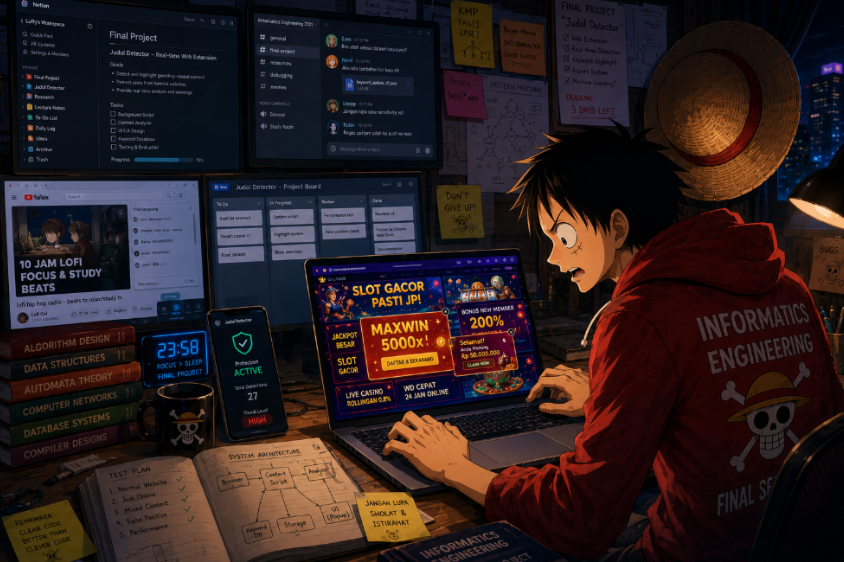
\includegraphics[width=0.6\textwidth]{01-pendahuluan/luffy-tugas.png}
        \caption{Luffy mengerjakan tugas (Sumber: AI Generated Image)}
    \end{center}
\end{figure}

Luffy adalah seorang mahasiswa Teknik Informatika yang sedang menjalani semester akhirnya bersama timnya. Setelah mempelajari berbagai materi selama masa perkuliahan, mereka mendapatkan tugas besar terakhir sebagai bentuk penerapan ilmu yang telah dipelajari. Luffy ingin membuat sebuah proyek yang tidak hanya memenuhi kebutuhan akademik, tetapi juga memiliki hubungan dengan permasalahan yang sering ditemui di kehidupan sehari-hari.

Saat menggunakan internet untuk belajar, mencari referensi, maupun membuka berbagai website, Luffy sering menemukan kemunculan iklan dan konten perjudian online yang tersebar di berbagai halaman web. Tidak jarang, konten tersebut menggunakan variasi penulisan yang unik dan tersamarkan agar sulit dikenali secara langsung. Dari situ, Luffy mulai tertarik untuk mempelajari bagaimana sebuah sistem dapat mengenali pola-pola tertentu pada teks secara otomatis dan efisien.

Berangkat dari ide tersebut, Luffy dan timnya memutuskan untuk mengembangkan sebuah browser extension bernama Judol Detector sebagai proyek tugas besar mereka. Melalui proyek ini, mereka berharap dapat menggabungkan konsep algoritma, pemrosesan string, dan pengembangan perangkat lunak ke dalam sebuah aplikasi yang interaktif dan aplikatif.

\begin{figure}[H]
    \begin{center}
        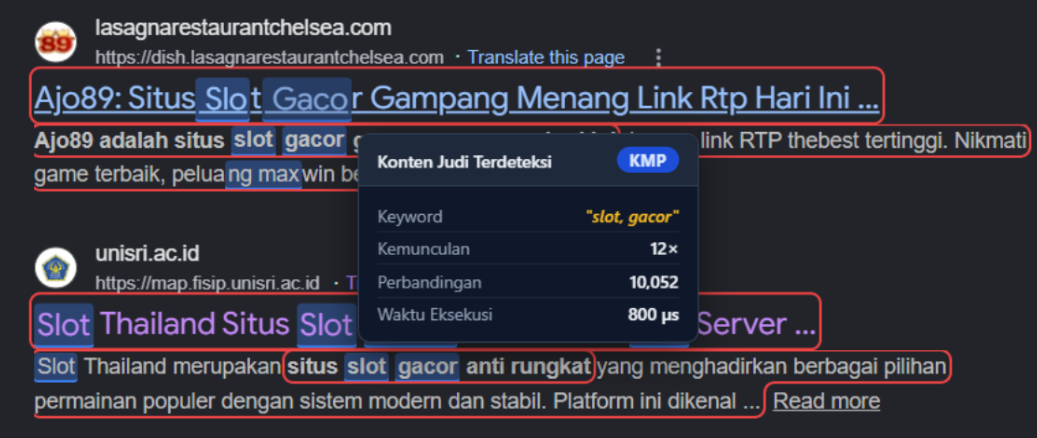
\includegraphics[width=0.6\textwidth]{01-pendahuluan/visualiasi.png}
        \caption{Visualisasi Browser Extension
            (Sumber: Asisten IRK)}
    \end{center}
\end{figure}

\section{Spesifikasi Wajib}
Pada tugas besar ini, buatlah sebuah chromium browser extension yang dapat mendeteksi informasi yang mengandung unsur judol. Sebagai catatan, seperti yang biasa kita temukan dalam website sekarang dengan format \texttt{<kata><angka>}. Contoh: \texttt{GACOR99, MAXWIN88, MADU308}, dan sebagainya. Sistem harus memiliki minimal fitur dengan detail seperti berikut.

\begin{enumerate}
    \item Extension yang dibuat pada tugas besar ini dikembangkan dengan bahasa Typescript. Dalam proses pencocokan kata kunci, sistem wajib mengimplementasikan algoritma Knuth-Morris-Pratt dan Boyer Moore serta RegEx. Untuk algoritma selain RegEx, pencarian dilakukan menggunakan file \texttt{keyword.txt} (file ini boleh dimodifikasi sesuai kebutuhan) yang dipisahkan dengan endline untuk melakukan string matching secara iterative, sehingga pengguna tidak memasukkan input, tapi sistem yang membaca file tersebut secara langsung.

          Untuk pencarian dengan regex, format pencarian seminimal mungkin dapat menghandle 2 atau 3 angka di belakang kata tanpa spasi. Contoh: MAXWIN234, SLOT99. Test case yang diberikan nanti akan sangat bervariasi, sehingga pastikan pencarian RegEx diimplementasikan dengan detail dan dapat menghandle banyak edge case. Adapun juga algoritma Aho-Corasick dan Rabin Karp apabila ingin mengerjakan bonus, sesuai tertera di Spesifikasi Bonus dibawah.

    \item Perlu diketahui bahwa, Developer Judol pun juga membuat penamaan dari websitenya, seperti pada teknik Phising, jadi membuat nama domain yang serupa dengan pada umumnya, namun nyatanya berbeda. Ini terjadi oleh karena adanya perbedaan kode komputer (unicode), dan komputer mengiranya adalah karakter yang berbeda.

          Maka dari itu, sistem harus bisa membaca kecocokan secara exact matching dan juga fuzzy matching (apabila tidak ditemukan kecocokan yang persis). Untuk setiap kata kunci yang tidak memiliki kemunculan sama sekali pada saat exact matching, lakukan pencarian kembali dengan perhitungan tingkat kemiripan menggunakan algoritma Weighted Levenshtein Distance. Penyesuaian bobot (weight) ini krusial karena pelaku sering kali menyiasati strategi dengan menggunakan huruf pengganti yang mirip secara visual (misalnya mengubah huruf 'O' menjadi angka '0', 'A' menjadi '4', atau 'I' menjadi '1'). Implementasi harus memperhatikan hal-hal berikut:

          \begin{enumerate}
              \item Weighted Cost: Berikan bobot penalti yang lebih kecil untuk substitusi karakter yang mirip secara visual dibandingkan dengan karakter yang benar-benar berbeda.
              \item Thresholding: Tentukan nilai ambang batas (threshold) kemiripan yang tepat untuk memastikan sistem tetap memberikan hasil yang relevan namun tetap menghindari munculnya false positive.
          \end{enumerate}
          Algoritma ini memungkinkan sistem untuk tetap menampilkan hasil pencarian yang relevan meskipun terdapat perbedaan minor, kesalahan ketik, atau upaya manipulasi teks oleh pengguna. Perlu diperhatikan bahwa secara konsep, exact matching juga merupakan bagian dari fuzzy matching.

          \[
              \operatorname{lev}(a,b)=
              \begin{cases}
                  |a|                                                                          & \text{if } |b|=0,                                         \\
                  |b|                                                                          & \text{if } |a|=0,                                         \\
                  \operatorname{lev}(\operatorname{tail}(a),\operatorname{tail}(b))            & \text{if } \operatorname{head}(a)=\operatorname{head}(b), \\
                  1+\min\{\,\operatorname{lev}(\operatorname{tail}(a),b),                                                                                  \\
                  \quad\,\operatorname{lev}(a,\operatorname{tail}(b)),                                                                                     \\
                  \quad\,\operatorname{lev}(\operatorname{tail}(a),\operatorname{tail}(b))\,\} & \text{otherwise.}
              \end{cases}
          \]

    \item Jadi sistem menjalan pengecekan dengan hirarki sebagai berikut:
          \begin{itemize}
              \item Exact Matching: Algoritma pattern matching untuk mencari kata kunci dasar dari \texttt{keyword.txt}.
              \item RegEx Matching: Secara paralel atau sekuensial, jalankan Regex untuk menangkap pola \texttt{<kata><angka>}.
              \item Fuzzy Matching: Kalau string dalam DOM tidak lolos namun memiliki kemiripan, jalankan dengan Weighted Levenshtein Distance dalam upaya manipulasi karakter
          \end{itemize}
    \item Apabila ditemukan result keyword, maka elemen DOM terkait harus ditandai, dengan warna bebas. Namun highlight tidak boleh merusak layout, tepat sasaran dan dapat terhapus saat rescanning.
    \item Saat user hover pada elemen yang terdeteksi, maka tampilkan tooltip dengan informasi berikut:
          \begin{itemize}
              \item Keyword yang terdeteksi
              \item Algoritma yang digunakan
              \item Jumlah kemunculan
              \item Waktu eksekusi
          \end{itemize}
          Tooltip dibuat dengan custom DOM element.
    \item Terdapat juga statistik secara realtime pada popup extension yang menampilkan:
          \begin{itemize}
              \item Total keyword yang ditemukan
              \item Perbandingan jumlah keyword yang satu dengan lainnya, menggunakan visualisasi
              \item Waktu eksekusi tiap algoritma
              \item Jumlah match tiap algoritma
          \end{itemize}
    \item Setiap kelompok harap mengisi nama kelompok dan anggotanya pada link berikut, paling lambat Minggu, 17 Mei 2026 23.59. Nama kelompok dilarang mengandung unsur SARA, penghinaan, provokasi, atau hal-hal lain yang bertentangan dengan norma hukum.

          Perlu diperhatikan bahwa kelompok tubes untuk mata kuliah ini tidak boleh sama. Jadi jika berkelompok dengan X pada tubes ini, maka pada tubes selanjutnya anda tidak diperkenankan berkelompok dengan X.

\end{enumerate}

\section{Persyaratan dan Larangan}
\begin{itemize}
    \item Seluruh algoritma string matching wajib dibuat from scratch
    \item Dilarang keras menggunakan
          \begin{itemize}
              \item \texttt{string.includes()}
              \item \texttt{string.indexOf()}
              \item Built-in search function
              \item External string matching library
          \end{itemize}
    \item Implementasi manual wajib mencakup:
          \begin{itemize}
              \item Border function
              \item Failure function
              \item Last occurrence table
              \item Shifting process
              \item Comparison Counting

          \end{itemize}
    \item Regex diperbolehkan menggunakan regex engine dari JavaScript.
\end{itemize}

\section{Spesifikasi Bonus}
\begin{enumerate}
    \item (6 poin) \textbf{[Video]} Membuat video tentang browser extension Judol Detector yang dikembangkan, kemudian mengunggahnya di Youtube. Video dibuat harus memiliki audio dan menampilkan wajah dari setiap anggota kelompok. Untuk contoh video tubes stima tahun-tahun sebelumnya dapat dilihat di Youtube dengan kata kunci “Tubes Stima”, “strategi algoritma”, “Tugas besar stima”, dll. Semakin menarik dan informatif video, maka semakin banyak poin yang diberikan.
    \item (4 poin) \textbf{[Algoritma Bonus]} Mengimplementasikan Algoritma Aho-Corasick dan Rabin Karp sebagai algoritma alternatif.
    \item (5 poin) \textbf{[Censorship / Blur Teks]} Mengimplementasikan fitur blur visual secara otomatis pada elemen halaman web yang terdeteksi memuat konten judi online. Tidak hanya sekadar menghighlight teks, ekstensi langsung melakukan aksi blur pada elemen yang mengandung kata kunci judol, sehingga konten tersebut tidak terlihat oleh pengguna. Perlu diperhatikan, terdapat toggle on/off untuk ini.
    \item (5 poin) \textbf{[Optical Character Recognition Pada Gambar]} Mengimplementasikan fitur OCR untuk mendeteksi kata kunci judi online yang sengaja disembunyikan dalam bentuk gambar. Ekstensi akan mengekstrak teks dari elemen gambar yang ditemukan di halaman, kemudian mencocokkannya dengan daftar kata kunci judol, lalu melakukan blur atau penggantian pada gambar yang terdeteksi mengandung konten judol. Fitur ini dapat diimplementasikan dengan Tesseract.js

\end{enumerate}
% Deskripsi tugas (dapat menyalin spesifikasi tugas ini).

\chapter{Landasan Teori}
\section{Pattern Matching}

\subsection{Algoritma Knuth-Morris-Pratt (KMP)}

\subsection{Algoritma Boyer-Moore}

\subsection{Algoritma Aho-Corasick}

\subsection{Algoritma Rabin-Karp}

\section{Regular Expression (RegEx) Matching}

\section{Fuzzy Matching}

\subsection{Weighted Levenshtein Distance}

\section{Optical Character Recognition (OCR)}

\section{Chromium Browser Extension}

\subsection{Arsitektur Singkat}

\subsection{Akuisisi dan Pemindaian DOM}

% Dasar teori algoritma Knuth-Morris-Pratt dan Boyer-Moore secara umum (serta algortima Aho-Corasick dan Rabin Karp  jika mengerjakan bonus).
% Penjelasan singkat mengenai browser extension yang dibangun.

\chapter{Analisis Pemecahan Masalah}
\input{sections/03-analisis-pengujian-masalah.tex}
% Langkah-langkah pemecahan masalah.
% Proses pemetaan masalah menjadi elemen-elemen algoritma KMP dan BM.
% Fitur fungsional dan arsitektur extension yang dibangun.
% Contoh ilustrasi kasus.

\chapter{Implementasi dan Pengujian}
% Section 4 — Implementasi dan Pengujian
\section{Implementasi dan Pengujian}

\subsection{Implementasi Sistem Deteksi}

\subsubsection{Alur Umum Eksekusi}
Content script menjadi titik awal eksekusi sistem. Saat halaman dibuka, script memuat daftar keyword, melakukan normalisasi teks, lalu meneruskan hasilnya ke pipeline pencarian. Pada tahap ini, pencarian exact dijalankan terlebih dahulu menggunakan KMP dan Boyer--Moore. Jika pola yang dicari juga sesuai dengan format tertentu, RegEx dipakai untuk menangkap variasi yang lebih terstruktur seperti kata diikuti dua atau tiga digit.

Jika exact matching tidak menemukan hasil yang memadai, sistem masuk ke jalur fallback fuzzy dengan Weighted Levenshtein. Jalur ini digunakan untuk menangkap variasi karakter yang mirip atau bentuk penulisan yang sedikit melenceng dari keyword asli. Setelah hasil ditemukan, modul rendering menerima data tersebut untuk menampilkan highlight, tooltip, dan statistik pada popup.

Seluruh alur tersebut dibuat berlapis agar hasil yang paling presisi didahulukan oleh exact matching, sementara fuzzy hanya dipakai saat benar-benar diperlukan. Dengan urutan ini, sistem tetap cepat untuk kasus umum, tetapi masih toleran terhadap variasi teks yang lebih sulit dikenali.

\subsubsection{Struktur Data dan Modul}
Implementasi sistem tersebar pada beberapa kelompok file utama. Folder \texttt{src/algorithms/*} berisi algoritma pencarian seperti KMP, Boyer--Moore, RegEx helper, dan Weighted Levenshtein. Folder \texttt{src/content/*} menangani pembacaan DOM, proses scanner, pembuatan highlight, tooltip, dan integrasi OCR bila fitur tersebut diaktifkan. Sementara itu, folder \texttt{src/popup/*} bertanggung jawab atas tampilan statistik dan kontrol interaksi pengguna.

Data hasil pencarian dibentuk menjadi struktur yang seragam agar bisa dipakai lintas modul. Struktur ini memuat keyword yang ditemukan, posisi atau index kemunculan, panjang match, nama algoritma yang dipakai, serta waktu eksekusi. Dengan format yang konsisten, hasil dari algoritma berbeda bisa langsung dibandingkan pada popup maupun pada tahap rendering di halaman.

Pemisahan data seperti ini juga membantu menjaga alur kerja tetap jelas. Scanner hanya fokus mengumpulkan kandidat, algoritma fokus melakukan pencocokan, dan renderer fokus menampilkan hasil. Pendekatan tersebut membuat proses debugging serta evaluasi hasil pengujian menjadi lebih mudah.

\begin{figure}[H]
  \centering
  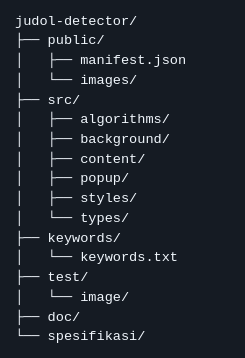
\includegraphics[width=0.95\linewidth]{../public/04-implementasi-pengujian/struktur.png}
  \caption{Diagram struktur data dan modul}
  \label{fig:code-structure}
\end{figure}

\subsubsection{Implementasi Exact Matching}
KMP digunakan sebagai salah satu algoritma exact matching utama karena memiliki struktur pencarian yang stabil dan efisien. Implementasinya dimulai dari pembentukan failure function atau border function untuk setiap keyword. Setelah itu, teks halaman dipindai dengan memanfaatkan informasi prefix yang sudah dihitung sebelumnya, sehingga perbandingan karakter yang tidak perlu bisa dihindari. Pada tahap ini, sistem juga mencatat jumlah perbandingan yang terjadi agar performa algoritma dapat dianalisis saat pengujian.

Boyer--Moore dipakai sebagai pembanding terhadap KMP karena pendekatannya berbeda dalam menangani mismatch. Algoritma ini membangun last-occurrence table untuk menentukan pergeseran saat karakter yang dibandingkan tidak cocok. Dalam kasus tertentu, terutama ketika pola yang dicari cukup pendek atau mismatch muncul jauh di dalam string, Boyer--Moore bisa melakukan pergeseran yang lebih besar dibandingkan scan linear biasa.

RegEx digunakan untuk menangkap bentuk teks yang lebih terstruktur, terutama pola yang terdiri dari kata dan dua atau tiga digit. Pola umum yang dipakai adalah format seperti \texttt{\textbackslash b([A-Za-z]+)(\textbackslash d\{2,3\})\textbackslash b}, sehingga keyword yang diikuti angka tetap bisa terdeteksi tanpa harus dituliskan satu per satu di daftar exact match. Pendekatan ini berguna untuk variasi seperti slot, win, atau gacor yang sering muncul dalam bentuk kombinasi huruf dan angka.

\subsubsection{Implementasi Fuzzy Matching}
Weighted Levenshtein dipakai sebagai mekanisme fuzzy matching untuk menangani teks yang mirip tetapi tidak identik dengan keyword. Bobot substitusi diberi perhatian khusus pada pasangan karakter yang sering tertukar, seperti O dan 0, A dan 4, I dan 1, serta E dan 3. Dengan bobot ini, perbedaan visual yang kecil tidak langsung dianggap sebagai mismatch besar.

Fuzzy matching tidak dijalankan sebagai langkah utama. Jalurnya hanya aktif ketika exact matching tidak menghasilkan hasil yang cukup, sehingga biaya komputasi bisa dijaga dan false positive tidak terlalu besar. Threshold juga disesuaikan agar sistem tidak terlalu longgar, tetapi tetap mampu menangkap variasi teks yang memang masih relevan dengan keyword target.

Pendekatan bertahap ini membuat fuzzy matching lebih aman dipakai. Exact matching tetap menjadi tulang punggung sistem, sedangkan fuzzy hanya berperan sebagai penyelamat untuk kasus variasi ejaan, unicode, atau substitusi karakter yang umum muncul di lapangan.

\subsubsection{Highlighting dan Tooltip}
Pemilihan target DOM dilakukan dengan hati-hati agar layout halaman tidak rusak. Sistem menargetkan text node yang aman untuk dibungkus atau diberi penanda visual, terutama pada elemen seperti paragraf dan span. Dengan cara ini, hasil highlight bisa terlihat jelas tanpa memaksa perubahan struktur elemen secara berlebihan.

Setiap kali re-scan dilakukan, highlight lama dihapus lebih dulu sebelum hasil baru ditampilkan. Mekanisme remove ini penting supaya tidak ada highlight ganda, tooltip lama, atau jejak hasil scan sebelumnya yang tertinggal di halaman. Selain menjaga kerapian tampilan, pendekatan ini juga memastikan hasil yang tampil benar-benar merepresentasikan scan terbaru.

Tooltip dipakai untuk menampilkan detail tambahan dari hasil deteksi. Informasi yang ditampilkan mencakup keyword yang ditemukan, algoritma yang memunculkan hasil tersebut, jumlah kemunculan, dan waktu eksekusi. Informasi ini membantu pengguna memahami mengapa sebuah teks ditandai, sekaligus memberi konteks ketika beberapa algoritma menghasilkan hasil yang berbeda.

\subsubsection{Statistik Popup}
Statistik popup menerima data hasil scan secara real-time melalui runtime messages atau storage sementara, tergantung kebutuhan sinkronisasi antarmodul. Setiap hasil yang dikirimkan akan direkap agar popup dapat menampilkan ringkasan deteksi tanpa perlu memindai ulang halaman.

Tampilan statistik difokuskan pada dua hal utama, yaitu jumlah temuan dan waktu eksekusi per algoritma. Dengan begitu, pengguna dapat melihat algoritma mana yang paling sering menemukan match dan algoritma mana yang paling cepat pada kondisi tertentu. Informasi ini juga menjadi dasar analisis pada bagian pengujian.

Selain ringkasan total, statistik juga dapat dipakai untuk membandingkan performa tiap algoritma pada scan terakhir. Jika diperlukan, data tersebut dapat dijadikan bahan evaluasi untuk menentukan algoritma yang paling cocok digunakan pada pola teks tertentu.

\subsubsection{Bonus}
Sebagai bonus, sistem dapat diperluas dengan Aho--Corasick atau Rabin--Karp. Aho--Corasick cocok bila jumlah keyword sangat banyak karena dapat melakukan multi-pattern matching secara efisien, sedangkan Rabin--Karp berguna saat pencocokan berbasis hash lebih praktis untuk beberapa skenario tertentu. Bagian ini cukup dijelaskan secara singkat bila fitur tersebut memang diimplementasikan.

Fitur censorship atau blur berfungsi sebagai lapisan visual tambahan pada hasil deteksi. Ketika toggle diaktifkan, elemen target diberi efek blur atau overlay sehingga konten sensitif tidak langsung terbaca. Mekanisme ini biasanya digabung dengan hasil scan yang sudah ada, sehingga blur dapat diterapkan atau dihapus berdasarkan status kontrol pengguna.

OCR digunakan untuk mengekstraksi teks dari gambar sebelum hasilnya dimasukkan ke pipeline pencarian utama. Alur ini diperlukan ketika keyword tidak muncul sebagai teks HTML biasa, tetapi tertanam di dalam gambar. Karena OCR dipengaruhi resolusi, kontras, dan noise visual, hasilnya perlu diuji lebih hati-hati dibandingkan pencarian teks biasa.

\subsection{Pengujian Unit}

\sloppy

\subsubsection{Metodologi Pengujian}
Metodologi pengujian pada implementasi akhir dilakukan melalui runner otomatis \texttt{test/test.ts}. Runner ini membaca dataset \texttt{test-cases.json}, lalu mengeksekusi tujuh kasus uji utama (TC-01 sampai TC-07) sebagai input ke pipeline deteksi yang sama dengan yang digunakan extension. Dengan pendekatan ini, pengujian tidak hanya memeriksa format test case, tetapi benar-benar mengukur perilaku algoritma inti pada data uji yang terstandar.

Eksekusi test dilakukan dari command line menggunakan \texttt{npx tsx test/test.ts}. Saat dijalankan, runner membentuk \textit{detection context} sintetis per kasus (URL, timestamp, satu target teks, dan metadata indeks), kemudian mengirimkan konteks tersebut ke setiap engine secara langsung, yaitu KMP, Boyer--Moore, Aho--Corasick, Rabin--Karp, RegEx, dan Weighted Levenshtein. Selain pengujian per engine, runner juga memanggil fungsi agregasi utama \texttt{runDetectionEnginesDetailed} untuk mendapatkan hasil gabungan pipeline serta timing setiap algoritma.

Inisialisasi pengujian dilakukan dengan mock minimal terhadap dependency extension yang biasanya tersedia di browser. Pada \texttt{test/test.ts}, objek \texttt{chrome.runtime.getURL} dan \texttt{fetch} di-stub agar pemuatan \texttt{keywords/keywords.txt} tetap berjalan pada lingkungan Node. Daftar keyword mock dibuat konsisten dengan kata-kata kunci inti (misalnya \texttt{slot}, \texttt{gacor}, \texttt{maxwin}, \texttt{jackpot}, \texttt{bocoran}, \texttt{daftar sekarang}, \texttt{togel}) agar perilaku engine saat test mendekati kondisi runtime extension.

Hasil evaluasi diklasifikasikan menggunakan metrik biner deteksi: TP, FP, FN, dan TN. Untuk tiap kasus, runner membandingkan \texttt{expected} dari \texttt{test-cases.json} dengan \texttt{actual} hasil pipeline (apakah ada match atau tidak). Klasifikasi ini digunakan untuk dua level analisis: (1) level pipeline gabungan dan (2) level masing-masing engine. Dengan begitu, laporan dapat menampilkan bukan hanya apakah test lulus, tetapi juga sumber kesalahan (misalnya false positive pada konteks ambigu atau false negative pada input dengan separator/noise).

Desain ini membuat unit test terhubung langsung ke fungsi-fungsi utama algoritma, bukan sekadar validasi statis string. Konsekuensinya, angka performa dan kualitas deteksi yang diperoleh dari \texttt{test/test.ts} dapat dipakai sebagai dasar analisis pada bagian hasil, termasuk perbandingan stabilitas antaralgoritma dan identifikasi area perbaikan preprocessing.

\subsubsection{Matriks Kasus Uji}
Semua kasus uji direpresentasikan dalam \texttt{test-cases.json} dan direplikasi di bawah sebagai panduan pelaporan. Setiap subsubsection berikut menampilkan field yang sama dengan object JSON: \texttt{id}, \texttt{category}, \texttt{input}, \texttt{expected}, \texttt{label}, dan \texttt{rationale}. Pada bagian ini tidak disertakan screenshot maupun tabel hasil per kasus, karena lampiran output dipisahkan pada subsection khusus setelah daftar kasus.

\subsubsection{TC-01 — Exact Match (True Positive)}
\textbf{ID}: TC-01 \\
\textbf{Category}: \texttt{exact\_match\_positive} \\
\textbf{Input}:
\begin{verbatim}Promo terbaru! Daftar sekarang dan raih jackpot slot gacor maxwin bocoran hari ini
\end{verbatim}
\textbf{Expected}: true \\
\textbf{Label}: Exact match promosi \\
\textbf{Rationale}: Kasus baseline. Mengukur apakah algoritma exact match dapat menemukan keyword promosi tanpa modifikasi.

\subsubsection{TC-02 — Exact Match Negative / Ambigu}
\textbf{ID}: TC-02 \\
\textbf{Category}: \texttt{exact\_match\_negative} \\
\textbf{Input}:
\begin{verbatim}Silakan cek slot parkir nomor 12 di area kampus untuk kendaraan tamu
\end{verbatim}
\textbf{Expected}: false \\
\textbf{Label}: Ambigu - non-promotional slot \\
\textbf{Rationale}: Mengukur false positive ketika kata ambiguitas muncul dalam konteks non-promosi.

\subsubsection{TC-03 — Random Capitalization}
\textbf{ID}: TC-03 \\
\textbf{Category}: \texttt{random\_capitalize} \\
\textbf{Input}:
\begin{verbatim}Cek sekarang sLoT gAcOr dan raih keuntungan besar!
\end{verbatim}
\textbf{Expected}: true \\
\textbf{Label}: Kapitalisasi acak \\
\textbf{Rationale}: Membedakan algoritma case-sensitive dari case-insensitive; menguji normalisasi kapitalisasi.

\subsubsection{TC-04 — Number Substitution (Leet)}
\textbf{ID}: TC-04 \\
\textbf{Category}: \texttt{number\_substitution} \\
\textbf{Input}:
\begin{verbatim}Bonus m4xw1n dan sl0t g4c0r siap dimainkan hari ini!
\end{verbatim}
\textbf{Expected}: true \\
\textbf{Label}: Substitusi angka (leet) \\
\textbf{Rationale}: Menguji normalisasi atau pre-processing untuk menangani penggantian huruf dengan angka/simbol.

\subsubsection{TC-05 — Fuzzy Separator / Karakter Sisipan}
\textbf{ID}: TC-05 \\
\textbf{Category}: \texttt{fuzzy\_separator} \\
\textbf{Input}:
\begin{verbatim}Promo s-l-o-t g.a.c.o.r cuma hari ini!
\end{verbatim}
\textbf{Expected}: true \\
\textbf{Label}: Karakter pemisah di antara huruf \\
\textbf{Rationale}: Menguji kemampuan menghapus separator dan mengenali keyword setelah normalisasi.

\subsubsection{TC-06 — Unicode Lookalike (Cyrillic Substitution)}
\textbf{ID}: TC-06 \\
\textbf{Category}: \texttt{unicode\_lookalike} \\
\textbf{Input}:
\begin{verbatim}[U+0455]l[U+043E]t g[U+0430]c[U+043E]r bocoran terpercaya
\end{verbatim}
\textbf{Expected}: true \\
\textbf{Label}: Cyrillic homoglyphs \\
\textbf{Notes}: \texttt{U+0430->a}, \texttt{U+043E->o}, \texttt{U+0435->e}, \texttt{U+0455->s}. \\
\textbf{Rationale}: Menguji kemampuan algoritma untuk menangani homoglyph Unicode; field `notes` berisi codepoint substitusi.

\subsubsection{TC-07 — Combined Evasion}
\textbf{ID}: TC-07 \\
\textbf{Category}: \texttt{combined\_evasion} \\
\textbf{Input}:
\begin{verbatim}Sl0T-G4C0R h4r1 1n1, daftar sekarang!
\end{verbatim}
\textbf{Expected}: true \\
\textbf{Label}: Kombinasi teknik evasi \\
\textbf{Notes}: teknik yang digabung: kapitalisasi acak, substitusi angka, separator. \\
\textbf{Rationale}: Kasus paling sulit yang menggabungkan beberapa teknik evasi; diferensiator utama antar-algoritma.

\subsubsection{Lampiran Output Unit Test (CLI)}
Subsection ini digunakan untuk melampirkan bukti output eksekusi \texttt{test/test.ts} dari command line. Karena output CLI ringkas, cukup digunakan satu screenshot gabungan yang menampilkan seluruh hasil TC-01 sampai TC-07.

\begin{figure}[H]
  \centering
  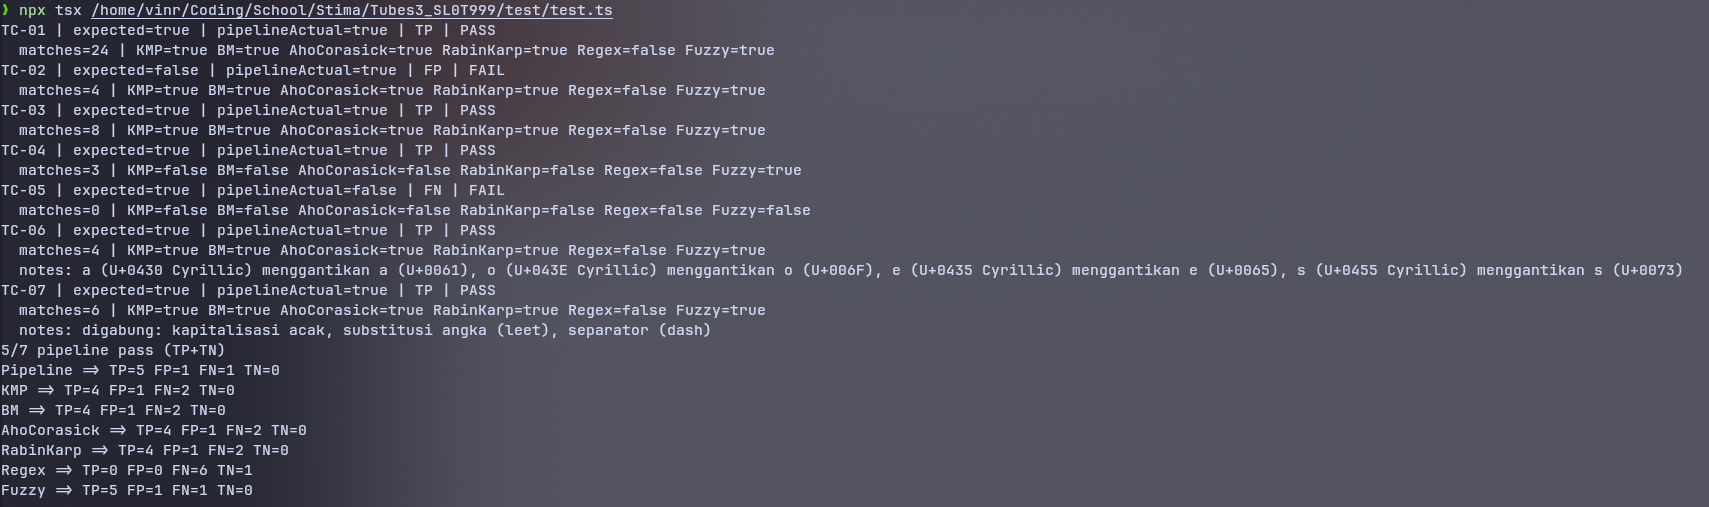
\includegraphics[width=0.95\linewidth]{../public/04-implementasi-pengujian/tc.png}
  \caption{Output CLI gabungan untuk seluruh test case unit}
  \label{fig:unit-cli-output}
\end{figure}

\begin{table}[H]
  \centering
  \resizebox{\linewidth}{!}{%
  \begin{tabular}{lccccccccc}
    \hline
    Test Case & Expected & Pipeline & KMP & BM & AhoCorasick & RabinKarp & RegEx & Fuzzy & Label \\
    \hline
    TC-01 & true & true & true & true & true & true & false & true & TP \\
    TC-02 & false & true & true & true & true & true & false & true & FP \\
    TC-03 & true & true & true & true & true & true & false & true & TP \\
    TC-04 & true & true & false & false & false & false & false & true & TP \\
    TC-05 & true & false & false & false & false & false & false & false & FN \\
    TC-06 & true & true & true & true & true & true & false & true & TP \\
    TC-07 & true & true & true & true & true & true & false & true & TP \\
    \hline
  \end{tabular}%
  }
  \caption{Perbandingan hasil setiap test case terhadap setiap algoritma (berdasarkan output CLI)}
\end{table}

\begin{table}[H]
  \centering
  \begin{tabular}{lrrrr}
    \hline
    Algoritma & TP & FP & FN & TN \\
    \hline
    Pipeline & 5 & 1 & 1 & 0 \\
    KMP & 4 & 1 & 2 & 0 \\
    Boyer--Moore & 4 & 1 & 2 & 0 \\
    AhoCorasick & 4 & 1 & 2 & 0 \\
    RabinKarp & 4 & 1 & 2 & 0 \\
    RegEx & 0 & 0 & 6 & 1 \\
    Weighted Levenshtein & 5 & 1 & 1 & 0 \\
    \hline
  \end{tabular}
  \caption{Ringkasan metrik TP/FP/FN/TN per algoritma dari output CLI}
\end{table}

\subsubsection{Format Pelaporan Hasil}
Format pelaporan hasil pada dokumen ini dibagi menjadi dua artefak utama: satu screenshot output CLI gabungan dan dua tabel ringkasan. Tabel pertama memuat perbandingan per test case terhadap seluruh algoritma, sedangkan tabel kedua merangkum metrik TP/FP/FN/TN per algoritma. Format ini dipilih agar pembaca dapat melihat bukti eksekusi dan ringkasan numerik tanpa pengulangan screenshot per kasus.

Jika ada kasus yang menghasilkan perilaku berbeda antaralgoritma, catatan singkat ditambahkan pada bagian analisis untuk menjelaskan penyebab teknisnya. Pendekatan ini menjaga pelaporan tetap ringkas, tetapi tetap kuat secara analitis.

\subsubsection{Analisis Hasil}
Analisis hasil difokuskan pada tiga hal utama. Pertama, perbandingan waktu eksekusi antara KMP, Boyer--Moore, dan RegEx. Kedua, evaluasi pengaruh threshold fuzzy terhadap false positive dan false negative. Ketiga, catatan keterbatasan sistem, misalnya pada OCR untuk gambar dengan resolusi rendah atau pada layout halaman yang sangat dinamis.

Perbandingan waktu sangat penting karena menunjukkan algoritma mana yang paling efisien pada jenis input tertentu. Sementara itu, evaluasi fuzzy membantu menjelaskan apakah peningkatan toleransi terhadap variasi teks sebanding dengan risiko deteksi yang salah. Kedua aspek ini harus dibahas bersama agar hasil pengujian tidak hanya bersifat deskriptif, tetapi juga analitis.

Bagian analisis juga dapat memuat pengamatan terhadap normalisasi teks. Jika normalisasi benar-benar memengaruhi hasil, maka hal tersebut perlu disebutkan secara eksplisit karena berdampak langsung pada jumlah match yang muncul di popup dan pada highlight yang terlihat oleh pengguna.

\subsection{Pengujian Integrasi}

Pengujian integrasi dilakukan untuk memverifikasi bahwa extension berfungsi sebagai produk utuh di browser, 
bukan hanya algoritma dalam isolasi. Fokus adalah pada injeksi content script, manipulasi DOM, rendering UI, 
dan manajemen state extension (enable/disable).

Berbeda dengan unit test yang menggunakan CLI runner, integration test menjalankan extension di browser Chromium/Chrome 
dan mengamati perilaku visual seperti highlight, badge popup, dan respons terhadap user action. Tes ini hanya menggunakan 
1 representative test case (TC-01 exact match) untuk menunjukkan end-to-end flow, bukan mengulangi semua 7 kasus.

\subsubsection{Skenario Pengujian Integrasi}

Pengujian integrasi mencakup dua skenario utama:

\begin{table}[H]
  \centering
  \renewcommand{\arraystretch}{1.2}
  \begin{tabular}{|p{2cm}|p{3cm}|p{4cm}|p{2cm}|}
    \hline
    \textbf{No} & \textbf{Skenario} & \textbf{Yang Diverifikasi} & \textbf{Input} \\
    \hline
    1 & Halaman berisi teks judol → badge/highlight muncul & End-to-end flow (DOM → content script → rendering) & TC-01 \\
    \hline
    2 & Teks judol di-load dinamis & Mutation observer menangkap DOM baru & Custom dynamic insert \\
    \hline
  \end{tabular}
  \caption{Matriks skenario pengujian integrasi extension}
\end{table}

\subsubsection{Metodologi dan Artefak Bukti}

\paragraph{Test Case 1 — End-to-End Flow (TC-01 Exact Match)}
Input HTML berisi teks promosi dengan multiple keyword dari TC-01. Saat halaman dibuka, sistem dipantau untuk memverifikasi:
(1) content script ter-inject tanpa error, (2) keyword ter-highlight pada halaman, (3) badge di popup menampilkan match count > 0, (4) waktu deteksi < 2 detik.

Bukti kesuksesan: screenshot halaman dengan highlights terlihat jelas, screenshot popup menampilkan detail per-algorithm.

\paragraph{Test Case 2 — Dynamic Content Loading}
Halaman awal tanpa keyword, kemudian keyword diinsert ke DOM via JavaScript. Sistem dipantau apakah mutation observer menangkap perubahan dan menampilkan highlight pada teks baru dalam < 500ms.

Bukti kesuksesan: screenshot sebelum dan sesudah DOM mutation, menunjukkan highlight muncul pada teks yang baru di-insert.

\subsubsection{Hasil Pengujian Integrasi}

\begin{figure}[H]
  \centering
  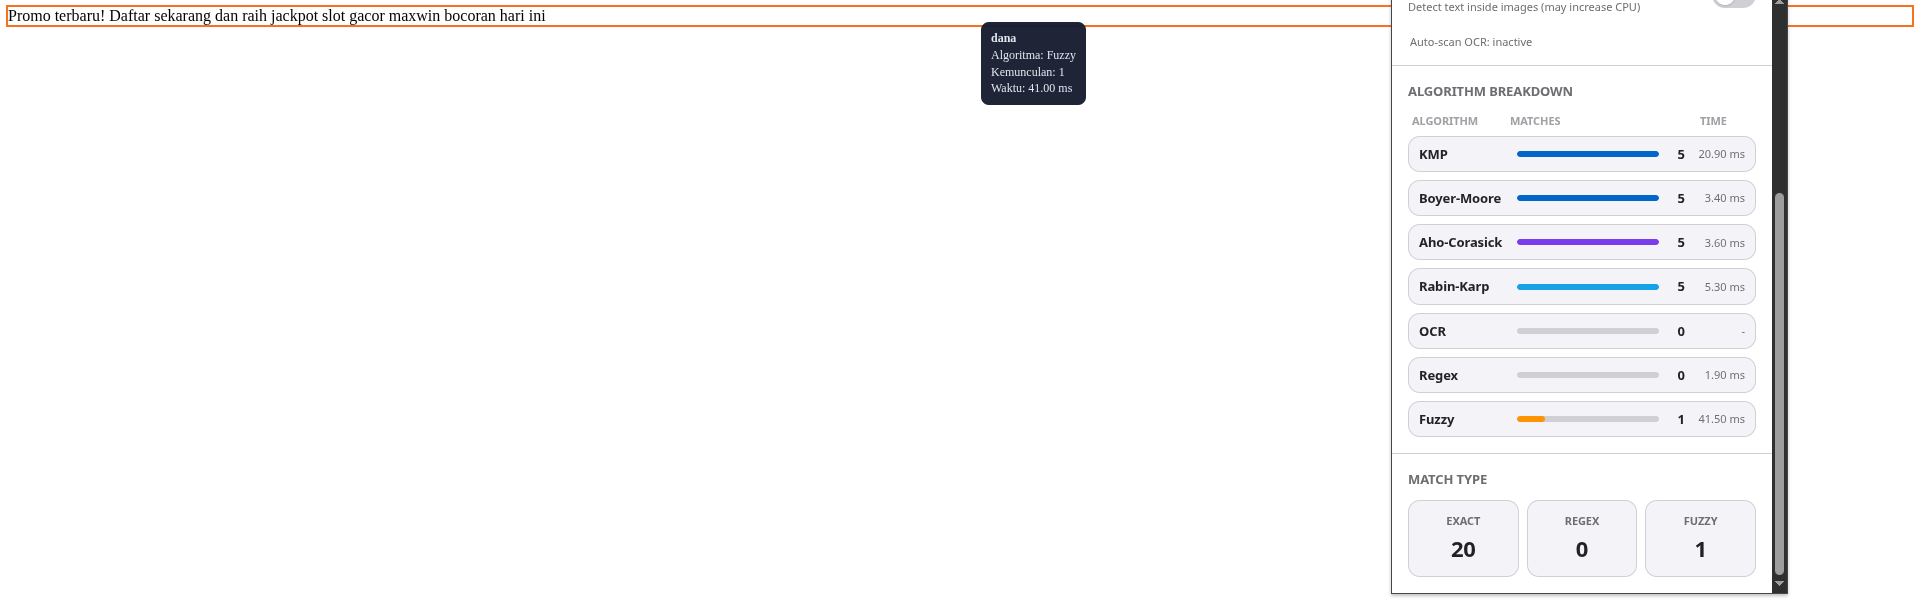
\includegraphics[width=0.95\linewidth]{../public/04-implementasi-pengujian/tc1-int.png}
  \caption{Hasil integrasi untuk skenario end-to-end TC-01}
  \label{fig:integration-tc1}
\end{figure}

\begin{figure}[H]
  \centering
  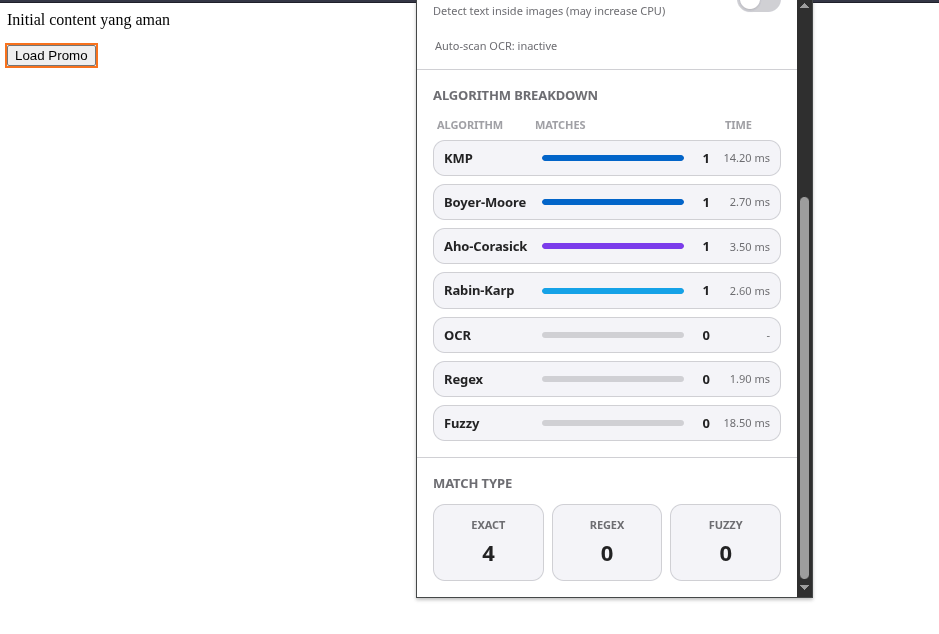
\includegraphics[width=0.95\linewidth]{../public/04-implementasi-pengujian/tc2-int-1.png}
  \caption{Hasil integrasi untuk skenario dynamic content - before}
  \label{fig:integration-tc2-before}
\end{figure}

\begin{figure}[H]
  \centering
  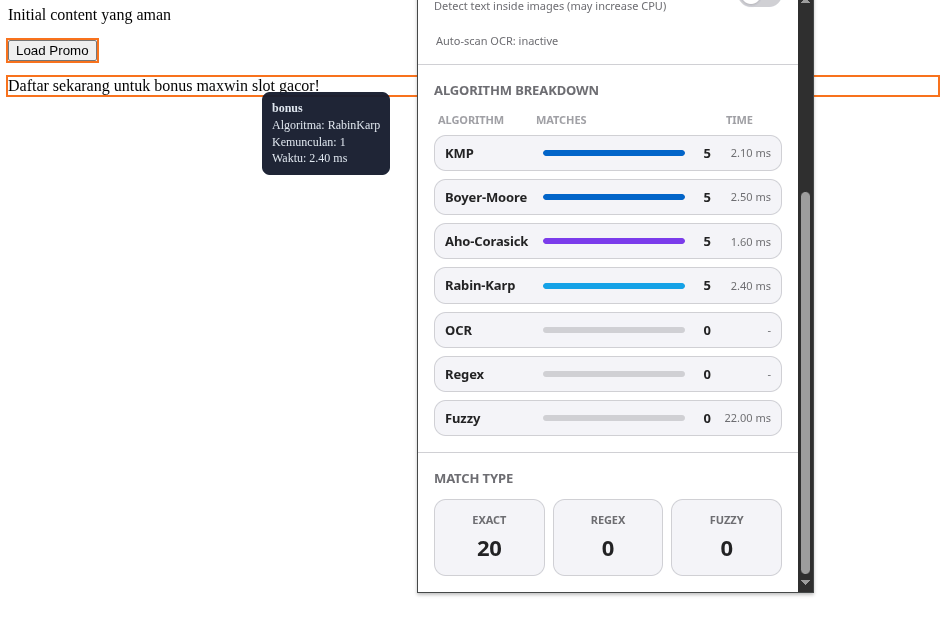
\includegraphics[width=0.95\linewidth]{../public/04-implementasi-pengujian/tc2-int-2.png}
  \caption{Hasil integrasi untuk skenario dynamic content - after}
  \label{fig:integration-tc2-after}
\end{figure}

\begin{table}[H]
  \centering
  \begin{tabular}{lc}
    \hline
    Skenario & Status \\
    \hline
    Test 1 (End-to-End) & ✓ PASS\\
    Test 2 (Dynamic Content) & ✓ PASS\\
    \hline
    \textbf{Total} & \textbf{2 PASS} \\
    \hline
  \end{tabular}
  \caption{Ringkasan hasil pengujian integrasi}
\end{table}

\subsubsection{Analisis Integrasi}

Pengujian integrasi memverifikasi bahwa komponen sistem yang testable di unit test juga berfungsi dengan baik dalam konteks browser. 
Test case 1 memastikan bahwa logika deteksi dari CLI dapat diteljur end-to-end di halaman nyata. Test case 2 menguji edge case DOM dinamis yang tidak tercakup oleh unit test.

Integrasi kedua skenario ini menunjukkan bahwa extension siap untuk uji coba di production environment atau QA lanjutan.

\section{Bonus: Blur Teks dan OCR}

\subsection{Blur/Censor Teks}
Fitur blur atau censorship dipakai untuk menyamarkan teks yang telah terdeteksi oleh sistem. Setelah deteksi dilakukan, elemen target menerima efek visual berupa blur atau overlay agar kontennya tidak langsung terbaca. Pendekatan ini dapat digunakan sebagai lapisan tambahan di atas proses highlight yang sudah ada.

\paragraph{Hasil Blur Before/After}
\begin{figure}[H]
  \centering
  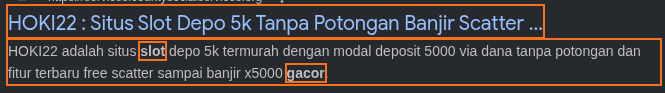
\includegraphics[width=0.95\linewidth]{../public/04-implementasi-pengujian/blur-1.png}
  \caption{Tampilan sebelum blur diterapkan}
  \label{fig:blur-before}
\end{figure}

\begin{figure}[H]
  \centering
  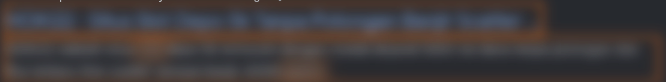
\includegraphics[width=0.95\linewidth]{../public/04-implementasi-pengujian/blur-2.png}
  \caption{Tampilan sesudah blur diterapkan}
  \label{fig:blur-after}
\end{figure}

Kontrol blur biasanya disediakan melalui popup sehingga pengguna dapat menyalakan atau mematikannya sesuai kebutuhan. Ketika mode blur diubah, sistem perlu melakukan re-scan atau pembaruan status agar elemen yang sebelumnya disamarkan dapat dikembalikan ke tampilan normal. Mekanisme ini penting supaya interaksi pengguna tetap fleksibel dan tidak mengganggu struktur halaman.

Pengujian blur dilakukan dengan membandingkan tampilan sebelum dan sesudah efek diterapkan. Selain memeriksa apakah teks benar-benar tersembunyi, perlu juga diperhatikan apakah efek blur memunculkan masalah layout seperti overflow, reflow, atau elemen lain yang ikut bergeser. Hasil ini akan membantu menilai apakah implementasi blur aman digunakan pada halaman nyata.

\subsection{OCR pada Gambar}
OCR digunakan untuk mengekstraksi teks dari gambar sebelum teks tersebut masuk ke pipeline scanning utama. Saat sistem menemukan gambar yang relevan, OCR engine dijalankan untuk membaca isi gambar dan mengubahnya menjadi teks yang bisa diproses seperti halnya konten HTML biasa. Dengan cara ini, keyword yang tidak muncul sebagai teks langsung tetap bisa ikut terdeteksi.

Sumber image uji yang digunakan pada subsection ini adalah \url{https://encrypted-tbn0.gstatic.com/images?q=tbn:ANd9GcRooMhQgXuCBMKAvTDiUkOVFU0UXwppZL6hyQ\&s}.

\paragraph{Hasil OCR Before/After}
\begin{figure}[H]
  \centering
  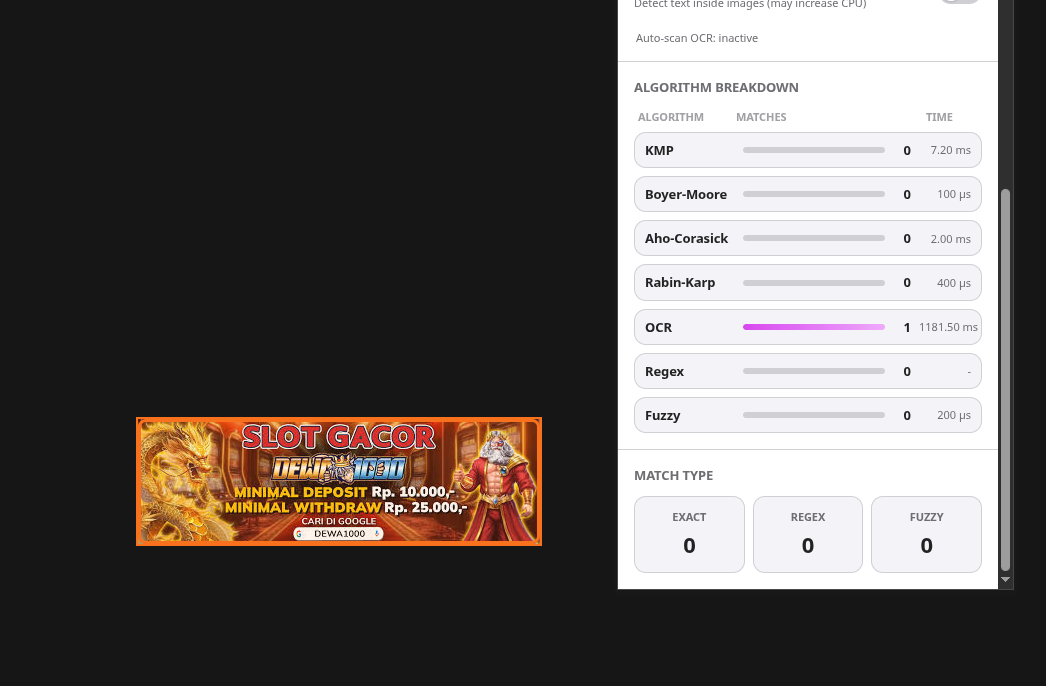
\includegraphics[width=0.95\linewidth]{../public/04-implementasi-pengujian/ocr-1.png}
  \caption{Gambar input sebelum OCR pada test/image/judol-3}
  \label{fig:ocr-before}
\end{figure}

\begin{figure}[H]
  \centering
  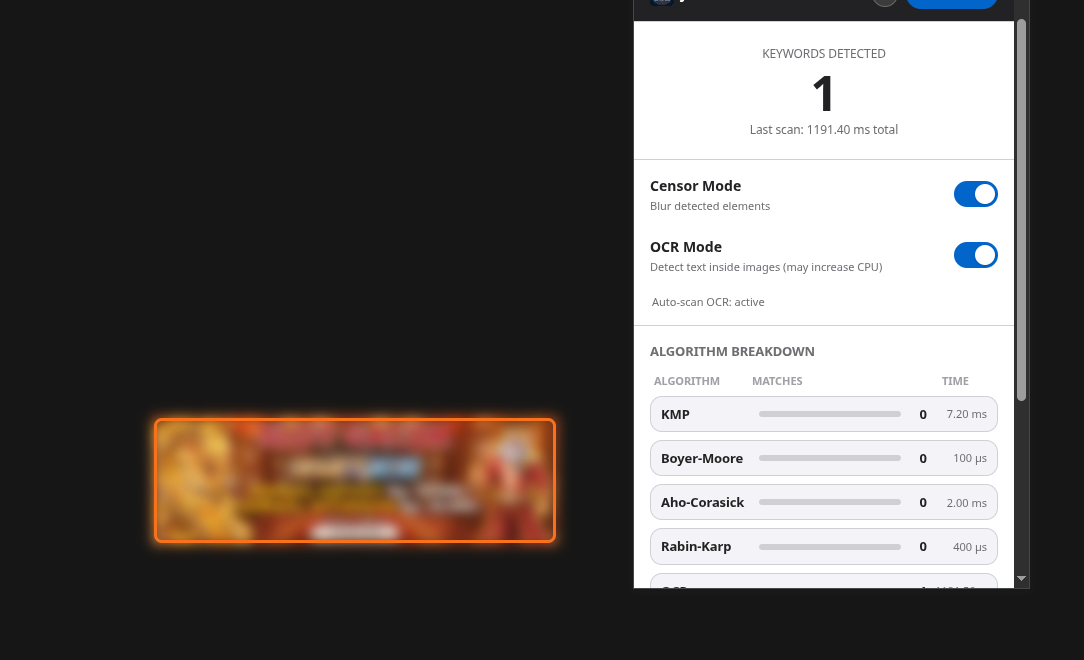
\includegraphics[width=0.95\linewidth]{../public/04-implementasi-pengujian/ocr-2.png}
  \caption{Hasil setelah OCR dieksekusi pada test/image/judol-3}
  \label{fig:ocr-after}
\end{figure}

Karena OCR bekerja pada citra, hasilnya sangat bergantung pada kualitas gambar. Resolusi rendah, noise, font dekoratif, atau kontras yang buruk dapat menurunkan akurasi ekstraksi. Oleh sebab itu, implementasi OCR perlu dibahas bersama dengan keterbatasannya agar pembaca memahami mengapa hasilnya mungkin tidak seakurat pencarian teks biasa.

Pengujian OCR sebaiknya dilakukan pada beberapa gambar dengan kualitas berbeda. Hasil ekstraksi teks dapat dibandingkan dengan ground truth untuk melihat seberapa baik OCR membaca keyword yang ditanam di dalam gambar. Selain akurasi, waktu pemrosesan per gambar juga perlu dicatat karena OCR biasanya lebih mahal secara komputasi dibandingkan matching pada teks biasa.

\section{Hasil Analisis}
\subsection{Perbandingan Kinerja Algoritma}
Berdasarkan output CLI, setiap test case memberikan pengaruh yang berbeda terhadap algoritma. Pada TC-01 (exact match promosi) dan TC-03 (kapitalisasi acak), hampir semua engine exact (KMP, Boyer--Moore, Aho--Corasick, Rabin--Karp) berhasil mendeteksi pola dengan konsisten. Ini menegaskan bahwa kekuatan utama algoritma exact ada pada kestabilan saat input masih dekat dengan bentuk canonical keyword.

TC-02 (konteks ambigu) menghasilkan false positive pada pipeline. Kasus ini menunjukkan bahwa kekuatan engine exact dalam menemukan literal string juga menjadi kelemahan ketika konteks semantik tidak dipertimbangkan. Dengan kata lain, TC-02 menyoroti bahwa perbaikan berikutnya perlu diarahkan ke context-aware filtering, bukan sekadar optimasi pencarian string.

TC-04 (number substitution) dan TC-07 (combined evasion) memperlihatkan peran dominan Weighted Levenshtein. Pada TC-04, seluruh engine exact gagal tetapi Fuzzy berhasil, sehingga strength utama Fuzzy terlihat jelas: toleransi tinggi terhadap substitusi karakter. Pada TC-07, engine exact kembali mampu mendeteksi karena masih ada token yang cukup dekat dengan keyword asli, sementara Fuzzy bertindak sebagai lapisan pengaman tambahan.

TC-05 (separator noise) menjadi false negative untuk seluruh engine dalam konfigurasi saat ini. Kasus ini sangat berpengaruh sebagai indikator bahwa preprocessing separator (misalnya normalisasi tanda hubung/titik/spasi antar karakter) masih menjadi bottleneck utama sistem. Jadi, TC-05 bukan hanya test gagal, tetapi test diagnostik yang menunjukkan area prioritas perbaikan.

TC-06 (unicode lookalike) berhasil dideteksi oleh sebagian besar engine pada setup saat ini, yang mengindikasikan bahwa normalisasi/tokenisasi yang dipakai masih memberi jalur deteksi untuk variasi unicode tertentu. Meski demikian, case ini tetap penting karena menguji batas robustnes terhadap homoglyph dan memverifikasi bahwa pipeline tidak hanya kuat di ASCII biasa.

Secara ringkas, strength masing-masing algoritma dapat dirangkum sebagai berikut: KMP dan Boyer--Moore kuat pada exact match cepat; Aho--Corasick kuat pada multi-keyword exact scanning; Rabin--Karp efektif sebagai exact matcher berbasis hash; RegEx kuat hanya jika pola sesuai definisi; Weighted Levenshtein unggul pada evasion berbasis substitusi/kemiripan karakter. Kombinasi test case TC-01 sampai TC-07 membuat kekuatan-kekuatan ini terlihat secara praktis, bukan hanya teoritis.

\subsection{Bagaimana Algoritma Saling Melengkapi}
Dilihat sebagai pipeline, TC-01 dan TC-03 mengonfirmasi bahwa lapisan exact matching memberikan fondasi presisi untuk kasus umum. TC-04 dan TC-07 menunjukkan bahwa lapisan fuzzy wajib dipertahankan untuk mengatasi teknik evasi. TC-05 menegaskan kebutuhan lapisan preprocessing yang lebih agresif sebelum exact/fuzzy dijalankan. TC-02 menegaskan kebutuhan lapisan context filtering setelah deteksi string ditemukan.

Urutan lapisan yang paling relevan dari hasil ini adalah: normalisasi teks, exact matching multi-engine, regex khusus pola terstruktur, fuzzy fallback, lalu context post-filter untuk menurunkan false positive. Dengan urutan ini, strength tiap algoritma tetap dimanfaatkan maksimal sambil mengurangi blind spot yang terungkap oleh test case.

Korelasi dengan fitur OCR juga tetap kuat. Hasil OCR cenderung membawa noise karakter; pada kondisi ini, engine exact dapat kehilangan match, sedangkan fuzzy bisa menjadi penyelamat. Sebaliknya, jika OCR menghasilkan token jelas, engine exact tetap lebih efisien. Jadi, hasil test case memperkuat keputusan desain bahwa kombinasi algoritma adalah kebutuhan struktural, bukan redundansi.

% Spesifikasi teknis program (struktur data, fungsi, dan prosedur yang dibangun).
% Penjelasan tata cara penggunaan extension (interface, fitur-fitur yang disediakan).
% Hasil pengujian minimal 5 kasus dengan variasi algoritma, dan jenis halaman yang berbeda.
% Analisis hasil pengujian dan perbandingan performa algoritma.

\chapter{Penutup}
\section{Kesimpulan}
Pada Milestone 1 ini, kelompok kami berhasil mengerjakan perancangan dan implementasi \textit{lexical analyzer} bahasa Arion berbasis DFA, mulai dari pemodelan state, implementasi modul lexer-token-main, hingga pengujian kasus dasar dan \textit{edge cases}. Program yang dihasilkan dapat membaca file input, mengenali token sesuai spesifikasi, serta melaporkan error leksikal dengan konsisten.

Tugas diselesaikan dengan alur yaitu, menerjemahkan spesifikasi ke desain DFA, mengimplementasikan kode secara modular, lalu memvalidasi melalui kumpulan test case. Pelajaran utama yang diperoleh adalah pentingnya dasar teori automata dalam pengembangan program ini, pentingnya pengujian kasus batas/\textit{edge cases}, dan pentingnya komunikasi tim agar integrasi kode serta dokumentasi berjalan lancar.

\section{Saran}

Untuk pengembangan lanjutan, disarankan memperkaya pesan error dengan menambahkan baris/kolom dimana kesalahan terjadi dan menyediakan mode debug transisi DFA. Dari sisi kerja tim, penggunaan alur \textit{branching} yang lebih intensif, \textit{code review} yang lebih terstruktur, dan standar penulisan yang konsisten akan meningkatkan kualitas hasil.

Sebagai langkah berikutnya, proyek dapat dilanjutkan ke analisis sintaksis dan semantik agar lexer yang telah dibangun menjadi fondasi compiler yang lebih lengkap.

% Kesimpulan dan saran.

\chapter{Lampiran}
\section{Pernyataan Tidak Melakukan Kecurangan}
Tugas ini disusun sepenuhnya tanpa bantuan kecerdasan buatan (Generative AI), melainkan hasil pemikiran dan analisis mandiri.
\begin{center}
    \begin{minipage}{\dimexpr\linewidth-2\fboxsep-2\fboxrule\relax}
        \hfill
        \begin{minipage}[t]{0.28\linewidth}\centering
            \vspace{-2pt}% adjust top alignment
            
\includegraphics[width=3cm]{public/ttd-vincent.jpeg}\\[4pt]
            Vincent Rionarlie\\
            13524031\\[12pt]

            
\includegraphics[width=3cm]{public/ttd-jason.png}\\[4pt]
            Jason Edward Salim\\
            13524034\\[12pt]

            
\includegraphics[width=3cm]{public/ttd-aufar.png}\\[4pt]
            Muhammad Aufar Rizqi Kusuam\\
            13524061
        \end{minipage}
    \end{minipage}%
\end{center}


\section{Tautan GitHub}
\href{https://github.com/Vixrlie/Tubes3_SL0T999}{Link GitHub}

\section{Tabel Checklist Spesifikasi}
\begin{center}
    \rowcolors{2}{gray!15}{white}
    \begin{tabularx}{\linewidth}{C{0.7cm} X C{1.0cm} C{1.0cm}}
        \toprule
        \textbf{No} & \textbf{Poin}                                                                                                                    & \textbf{Ya} & \textbf{Tidak} \\
        \midrule
        1           & Extension berhasil di-build dan di-load tanpa kesalahan pada Chromium browser dan dikembangkan dengan TypeScript                 &             &                \\
        2           & KMP dan Boyer-Moore diimplementasikan from scratch                                                                               &             &                \\
        3           & Regex meng-handle format \textless kata\textgreater\textless angka\textgreater dan berbagai edge case                            &             &                \\
        4           & Pencarian KMP \& BM membaca `keywords.txt` secara iteratif dan tidak menggunakan built-in search function atau library eksternal &             &                \\
        5           & Exact matching dan fuzzy matching berjalan benar                                                                                 &             &                \\
        6           & Elemen DOM terdeteksi diberi highlight dan terhapus saat rescanning                                                              &             &                \\
        7           & Tooltip muncul saat hover dengan informasi keyword, algoritma, kemunculan, dan waktu eksekusi                                    &             &                \\
        8           & Popup menampilkan statistik realtime (total keyword, perbandingan, waktu eksekusi, jumlah match)                                 &             &                \\
        9           & [Bonus] Membuat Video YouTube (jika dikerjakan)                                                                                  &             &                \\
        10          & [Bonus] Implementasi Algoritma Aho-Corasick dan Rabin-Karp                                                                       &             &                \\
        11          & [Bonus] Implementasi Censorship / Blur Teks dengan toggle on/off                                                                 &             &                \\
        12          & [Bonus] Implementasi Optical Character Recognition pada Gambar                                                                   &             &                \\
        \bottomrule
    \end{tabularx}
\end{center}

\section{Tabel Kontribusi}
\begin{center}
    \rowcolors{2}{gray!15}{white}
    \begin{tabularx}{\linewidth}{C{0.8cm} Y C{2.8cm} Y C{2.2cm}}
        \toprule
        \textbf{No} & \textbf{Nama Lengkap}       & \textbf{NIM} & \textbf{Deskripsi Pekerjaan}                                                                      & \textbf{Persentase Kontribusi (\%)} \\
        \midrule
        1           & Vincent Rionarlie           & 13524031     & Pembuatan algoritma pemrosesan string, bonus algortima Aho-Corasick dan Rabin-Karp, laporan akhir & 34                                  \\
        2           & Jason Edward Salim          & 13524034     & Pembuatan FE beserta dengan build-up nya, bonus censoring, laporan akhir                          & 33                                  \\
        3           & Muhammad Aufar Rizqi Kusuam & 13524061     & Pembuatan Controller program (Scanner, highlighter, DOM Integration, dll), laporan akhir          & 33                                  \\
        \bottomrule
    \end{tabularx}
\end{center}

% Isi kolom "Deskripsi Pekerjaan" dan persentase sesuai pembagian kerja sebenarnya.
% Pernyataan Tidak Melakukan Kecurangan
% Tautan repository Github 
% Tautan Video (jika mengerjakan bonus)
% Tabel Checklist Spesifikasi
% Tabel Pembagian Tugas


\nocite{*}
\bibliography{dafpus}

\end{document}
